\documentclass[11pt,a4paper]{article}
\usepackage[T1]{fontenc}
\usepackage[utf8]{inputenc}
\usepackage{lmodern}
\usepackage[margin=25mm,headheight=15pt]{geometry}
\usepackage{microtype}
\usepackage{amsmath,amssymb}
\usepackage{graphicx}
\usepackage{booktabs,longtable,array,tabularx}
\usepackage{enumitem}
\usepackage{fancyhdr}
\usepackage{caption}
\usepackage{xcolor}
\usepackage{tikz}
\usetikzlibrary{arrows.meta,positioning,calc}
\usepackage[hidelinks]{hyperref}
\hypersetup{pdftitle={PointNeuron 2 Progress and the Next Experimental Direction},pdfauthor={Jad Sawan}}
\graphicspath{{figures/}}
\definecolor{pnblue}{HTML}{395F7D}
\definecolor{pnteal}{HTML}{2B776D}
\definecolor{pnorange}{HTML}{956B38}
\definecolor{pnpurple}{HTML}{74528B}
\pagestyle{fancy}
\fancyhf{}
\fancyhead[L]{\small PointNeuron 2 Research Progress}
\fancyhead[R]{\small Jad Sawan}
\fancyfoot[C]{\thepage}
\renewcommand{\headrulewidth}{0.4pt}
\setlength{\parindent}{0pt}
\setlength{\parskip}{6pt}
\linespread{1.10}
\setlength{\emergencystretch}{2em}
\clubpenalty=10000
\widowpenalty=10000
\setcounter{tocdepth}{1}
\setcounter{secnumdepth}{2}
\setlist[itemize]{topsep=3pt,itemsep=3pt,parsep=0pt}
\setlist[enumerate]{topsep=4pt,itemsep=8pt,parsep=2pt,leftmargin=*}
\captionsetup{font=small,labelfont=bf,justification=justified,singlelinecheck=false,skip=7pt}
\renewcommand{\arraystretch}{1.15}
\newcommand{\seg}{\text{segment}}
\newcommand{\res}{\text{resampled}}
\newcommand{\evidence}[1]{~\cite{#1}}
\newcommand{\sourcepath}[1]{\href{https://github.com/GraphiCortex/PointNeuron_Rec/blob/8c363d3cc3a9c7698d367aa93b9b5d0ce0f63103/#1}{\nolinkurl{#1}}}
\tikzset{stage/.style={draw=pnblue!80,fill=pnblue!5,rounded corners=2pt,align=center,font=\small,minimum height=9mm,text width=57mm,inner sep=4pt},
 planned/.style={stage,draw=pnorange!90,dashed,fill=pnorange!4},
 learning/.style={stage,draw=pnpurple!80,fill=pnpurple!5},
 feedback/.style={stage,draw=pnteal!85,dashed,fill=pnteal!5},
 arr/.style={-{Latex[length=2mm]},line width=.55pt},
 lab/.style={font=\scriptsize,align=center,fill=white,inner sep=1pt}}
\newcommand{\DevelopmentMacroRows}{%
Classical graph & 54.33 & 69.14 & 47.43 & 54.72 & 0.918 \\
Archive leader\textsuperscript{*} & 64.00 & 73.12 & 58.72 & 68.14 & 1.250 \\
Broad dense head & 36.04 & 67.54 & 16.42 & 21.58 & 6.236 \\
Sato point forest & 38.49 & 63.13 & 20.08 & 24.93 & 6.204 \\
}
\newcommand{\DevelopmentNeuronRows}{%
\multicolumn{6}{l}{\textbf{SLP fly}}\\[2pt]
Classical graph & 39.21 & 55.34 & 18.66 & 23.74 & 3.743 \\
Archive leader\textsuperscript{*} & 77.23 & 91.25 & 70.15 & 86.19 & 0.915 \\
Broad dense head & 15.38 & 38.38 & 6.96 & 9.06 & 18.655 \\
Sato point forest & 25.61 & 56.74 & 13.29 & 16.98 & 9.574 \\
\midrule
\multicolumn{6}{l}{\textbf{Frog}}\\[2pt]
Classical graph & 50.22 & 72.86 & 45.30 & 54.78 & 0.331 \\
Archive leader\textsuperscript{*} & 70.46 & 81.31 & 63.99 & 75.06 & 0.720 \\
Broad dense head & 50.77 & 86.03 & 24.23 & 30.34 & 4.453 \\
Sato point forest & 56.42 & 80.09 & 33.54 & 40.06 & 2.396 \\
\midrule
\multicolumn{6}{l}{\textbf{Human Allen}}\\[2pt]
Classical graph & 61.74 & 73.20 & 55.74 & 61.51 & 0.778 \\
Archive leader\textsuperscript{*} & 68.92 & 76.18 & 65.25 & 71.15 & 1.606 \\
Broad dense head & 30.60 & 58.82 & 15.39 & 20.22 & 6.688 \\
Sato point forest & 25.86 & 45.19 & 13.85 & 17.16 & 8.498 \\
\midrule
\multicolumn{6}{l}{\textbf{Series017}}\\[2pt]
Classical graph & 74.82 & 85.41 & 69.50 & 79.41 & 0.696 \\
Archive leader\textsuperscript{*} & 0.00 & 0.00 & 0.00 & 0.00 & 0.000 \\
Broad dense head & 34.02 & 64.42 & 14.96 & 19.37 & 7.559 \\
Sato point forest & 29.83 & 55.86 & 14.96 & 17.99 & 8.225 \\
\midrule
\multicolumn{6}{l}{\textbf{Mouse RGC}}\\[2pt]
Classical graph & 61.93 & 83.35 & 57.07 & 70.97 & 0.655 \\
Archive leader\textsuperscript{*} & 82.11 & 91.43 & 76.88 & 87.96 & 1.147 \\
Broad dense head & 53.09 & 87.78 & 25.13 & 31.01 & 4.147 \\
Sato point forest & 50.65 & 75.82 & 29.63 & 37.09 & 2.820 \\
\midrule
\multicolumn{6}{l}{\textbf{Adult zebrafish}}\\[2pt]
Classical graph & 5.95 & 17.11 & 5.40 & 7.98 & 1.951 \\
Archive leader\textsuperscript{*} & 61.27 & 75.77 & 55.27 & 69.13 & 0.902 \\
Broad dense head & 17.18 & 49.77 & 11.13 & 21.14 & 5.747 \\
Sato point forest & 12.30 & 32.90 & 8.15 & 14.52 & 7.798 \\
\midrule
\multicolumn{6}{l}{\textbf{Janelia fly}}\\[2pt]
Classical graph & 86.43 & 96.69 & 80.31 & 84.62 & 0.742 \\
Archive leader\textsuperscript{*} & 88.03 & 95.89 & 79.52 & 87.49 & 0.997 \\
Broad dense head & 51.23 & 87.58 & 17.10 & 19.89 & 6.951 \\
Sato point forest & 68.74 & 95.32 & 27.14 & 30.69 & 4.347 \\
}
\newcommand{\OracleRows}{%
Original union & 90.42 & 95.67 & 41.49 & 46.19 & 2.398 \\
Compact union & 88.52 & 95.10 & 64.80 & 72.54 & 1.185 \\
Classical prune only & 64.77 & 77.01 & 58.58 & 64.74 & 0.491 \\
Classical prune plus add & 68.56 & 80.43 & 61.74 & 68.54 & 0.551 \\
}


\begin{document}
\hypersetup{pageanchor=false}
\begin{titlepage}
\centering
\vspace*{29mm}
{\LARGE\bfseries PointNeuron 2\par}
\vspace{6mm}
{\Large Progress and the Next Experimental Direction\par}
\vspace{10mm}
{\large From the original proposal to the current reconstruction experiments\par}
\vspace{25mm}
{\large Research Report\par}
\vspace{15mm}
{\large Jad Sawan\par}
\vspace{5mm}
{\large American University of Beirut\par}
\vfill
{\large Prepared for Dr Arij\par}
\vspace{8mm}
{\large 7 November 2026\par}
\vspace*{18mm}
\end{titlepage}
\hypersetup{pageanchor=true}
\pagenumbering{arabic}

\section*{Summary}
\addcontentsline{toc}{section}{Summary}
Since the earlier proposal, I have been trying to establish where the proposed changes to PointNeuron can actually improve a reconstructed neuron. The initial idea was to retain a point-based representation, prepare the image more carefully, learn stronger features with PointNeXt, use a Transformer to predict skeleton nodes, and learn their connections with GATv2. The semi-automatic part of the idea was also important: preparation could be reviewed before the image entered the rest of the pipeline, and eventually improve from the corrections made within a laboratory.

I started with the automatic path so that we could see what the system preserved, what it lost, and how much of any improvement came from learning. This led to a sequence of increasingly specific tests. First, I checked the image-to-point preparation and the model interfaces. Then I tested whether the proposal model could fit a small training problem. After that, I examined whether accurate node prediction was the right immediate target, and introduced a separate experiment with supervision against continuous reference curves.

There has been progress on those questions. A geometric-query Transformer matched all 178 target nodes in the four training boxes used for its fitting test. Input audits also showed that much of the reference structure lies near the sampled points. However, those findings did not carry through to a useful learned reconstruction. The later dense curve-head experiment, trained on 460 boxes from 33 neurons, reached development segment F1 of 36.04\% at two voxels and 67.54\% at six. The matched classical graph reached 54.33\% and 69.14\%.\evidence{transformer,support,broad}

The most useful change in my understanding came from looking at the reconstructed curves rather than node locations alone. A graph can lie near much of the reference while containing redundant paths and far too much length. Once we added one-to-one matching on uniformly resampled skeletons, the broad learned graph scored 16.42\% at two voxels, with 6.24 times the reference length. This made the remaining problem much more concrete: retaining useful structure while selecting a compact and well-connected reconstruction.\evidence{compact}

I therefore explored stronger image-derived candidates and simpler graph selectors before attempting GATv2. Those selectors also failed their agreed criteria. Reference-assisted editing experiments nevertheless found a feasible reconstruction at 61.74\% resampled F1 at two voxels. This is enough to motivate discussing an editing formulation, although it is not a learned result or a solved ceiling. A stronger archive tracer also narrows the apparent margin, and a coordinate-screen limitation still affects that comparison.\evidence{trees,post,benchmark}

My current inclination is to test the semi-automatic idea in a small, controlled way before asking you to approve a larger architectural change. In particular, I would like to find out whether sparse corrections improve preparation, and whether corrections on earlier neurons improve later, uncorrected neurons from the same acquisition group. The point-based representation, Transformer and GATv2 remain research components whose roles we should decide together. The experimental Transformer bypass described below has not been adopted as a replacement for the proposal we discussed.

\clearpage
\tableofcontents
\clearpage

\section{Where we started and what the changes were meant to achieve}
The starting point was PointNeuron's separation of geometry and connectivity. Instead of treating the entire microscopy stack as a dense voxel prediction problem, the image is represented by points. The original framework learns point features with DGCNN, predicts local skeleton centres through a proposal module, consolidates the proposals, and learns connectivity with a graph autoencoder. This was the part of the approach I wanted to retain: the representation makes the geometry explicit, while the graph stage gives us a place to reason about how branches connect.\evidence{pointneuron}

The proposed PN2 changes were intended to strengthen those responsibilities. PointNeXt would provide the image-point features. A Transformer would give proposal generation more context than a local prediction alone. GATv2 would learn how candidate nodes should connect. Better preparation would help the downstream models receive evidence from dim and thin processes, rather than mostly the strongest image structures. None of these substitutions, by itself, guaranteed a better final neuron; the experiments were meant to establish whether their expected benefits survived through the pipeline.\evidence{design}

The original semi-automatic idea fits at the beginning of this process. Before reconstruction, the user would see the image together with the prepared evidence and could indicate a region that had been missed or an area receiving too much attention. That is different from asking the user to trace the final skeleton manually. The longer-term aim would be for those corrections to improve preparation on subsequent images from the same laboratory.

For the fresh PN2 experiments, I kept that interaction deferred and tested the automatic path first. Otherwise, an improvement could come from additional manual information without telling us whether the learned reconstruction had improved. Figure~\ref{fig:original} shows the intended architecture against which the experiments should be read.

\begin{center}
\begin{minipage}{\linewidth}
\centering
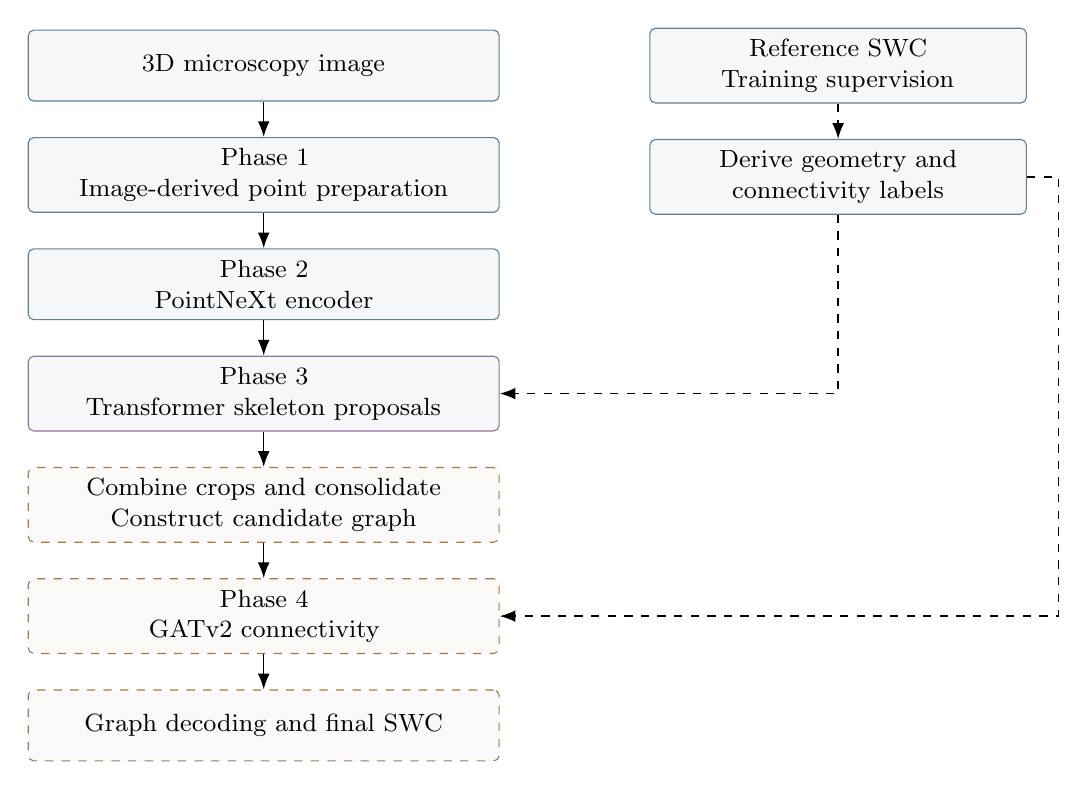
\begin{tikzpicture}[node distance=4.5mm and 16mm]
\node[stage] (image) {3D microscopy image};
\node[stage,below=of image] (prep) {Phase 1\\Image-derived point preparation};
\node[stage,below=of prep] (enc) {Phase 2\\PointNeXt encoder};
\node[learning,below=of enc] (trans) {Phase 3\\Transformer skeleton proposals};
\node[planned,below=of trans] (merge) {Combine crops and consolidate\\Construct candidate graph};
\node[planned,below=of merge] (gat) {Phase 4\\GATv2 connectivity};
\node[planned,below=of gat] (decode) {Graph decoding and final SWC};
\node[stage,right=19mm of image,text width=45mm] (ref) {Reference SWC\\Training supervision};
\node[stage,below=of ref,text width=45mm] (targets) {Derive geometry and\\connectivity labels};
\draw[arr] (image)--(prep);\draw[arr] (prep)--(enc);\draw[arr] (enc)--(trans);
\draw[arr] (trans)--(merge);\draw[arr] (merge)--(gat);\draw[arr] (gat)--(decode);
\draw[arr,dashed] (ref)--(targets);
\draw[arr,dashed] (targets.south) |- (trans.east);
\draw[arr,dashed] (targets.east) -- ++(4mm,0) |- (gat.east);
\end{tikzpicture}
\captionof{figure}{The intended PN2 architecture. Dashed supervision paths are used in training, not to select inference points or connections. The orange stages include whole-image work and learned connectivity that have not yet been completed. Optional review of preparation was part of the original semi-automatic idea, but was not used to repair the automatic results reported here.}
\label{fig:original}
\end{minipage}
\end{center}

\section{Establishing what reaches the model}
\subsection{The cohort and the meaning of development results}
Before training more broadly, I fixed a neuron-level working cohort from Gold166 and checked the capacity of the crop and target representation. This cohort contains 33 training neurons, seven development neurons and eight reserved neurons; it is not an evaluation of the entire Gold166 collection. There are 460 reference-present training boxes and 151 reference-present development boxes. The remaining boxes in the image grids are annotation-unknown; they were not treated as examples of biological background.\evidence{cohort}

The seven development neurons have been inspected repeatedly during this work. They also appeared in historical PN1 work. They supply no gradients to the fresh PN2 fits discussed here, but they are not an untouched final test. Their value at this stage is in identifying failures and comparing formulations. The eight reserved neurons have not had their source images or reference annotations opened for these experiments. They remain available for a later frozen evaluation.\evidence{cohort}

This distinction matters because a successful debugging result, a successful fit and a final generalization result answer different questions. I have kept them separate throughout the interpretation below.

\subsection{Point preparation preserved opportunity but not a guarantee}
The first question was whether the automatic preparation removed too much information before a learned model had any opportunity to use it. The preparation works from the image itself, preserving source coordinates and intensities in cached point packets. Reference traces are read for supervision and evaluation, not to select those ordinary inference points.

The saved audit found that, on development data, 70.24\% of reference length was within two voxels of an input point at 2,048 points per box; this rose to 91.98\% at 8,192 points. The apparent thin/dim stratum improved from 40.56\% to 83.23\%. Figure~\ref{fig:support} shows why point allocation remains relevant, even though it cannot explain every later error.\evidence{support}

\begin{figure}[htbp]
\centering
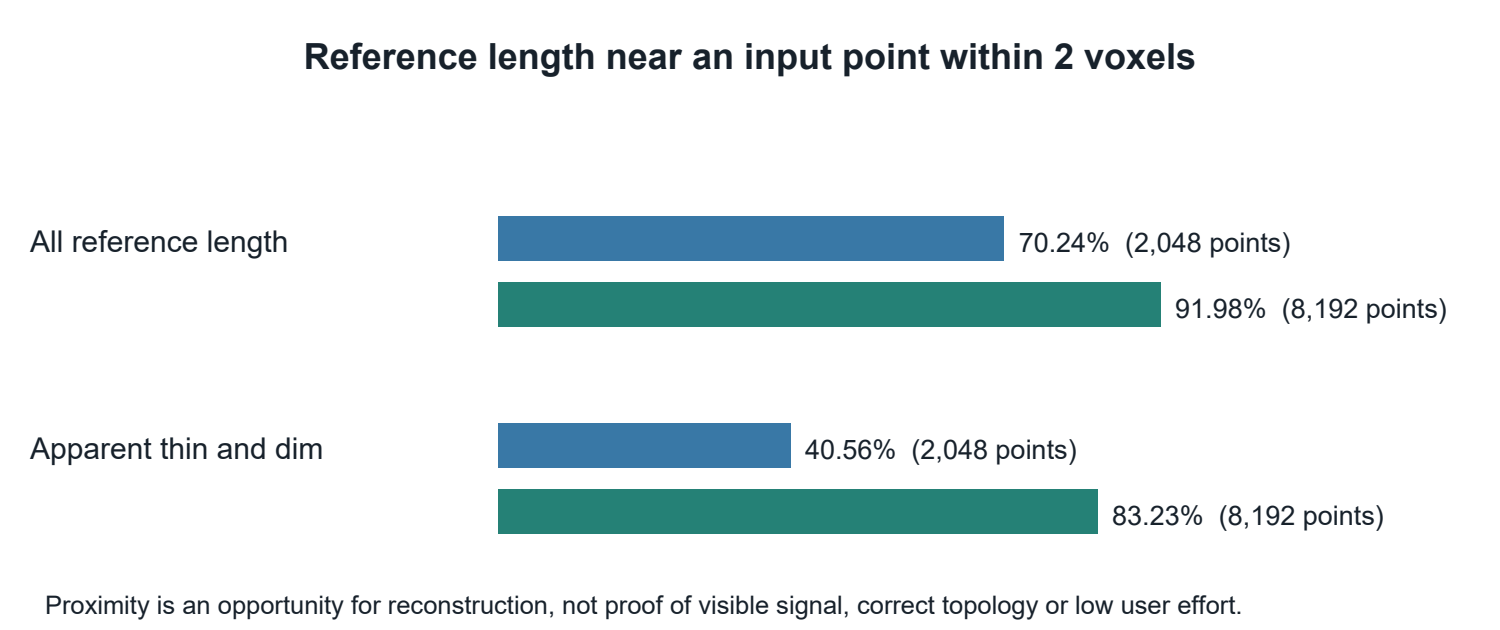
\includegraphics[width=\linewidth]{input_support.png}
\caption{Saved development input-support measurements. Increasing the point count provides more nearby evidence, particularly around thin/dim reference structure. These percentages measure proximity to points; they do not establish that the local image signal is informative or that a model will retain it.}
\label{fig:support}
\end{figure}

These findings gave me a reason to preserve the preparation infrastructure instead of restarting it. They did not qualify Phase 1 as complete in the stronger biological sense. A branch may have nearby points but weak signal, or may receive too few informative points at the working budget. Conversely, a well-sampled branch can still be lost by the proposal or selection stage. That became important in the later comparisons.

\section{First testing whether the proposal model could learn}
I initially tested the model on a small training task so that we could distinguish an implementation problem from a generalization problem. These tests were deliberately limited. They checked whether the input representation, PointNeXt features, query construction and losses could produce the intended target positions under ordinary inference.

One useful result came from the geometric-query Transformer. On the four training boxes, it matched all 178 target nodes within two voxels and produced zero accepted extras at the fixed cutoff. Train/evaluation consistency also passed. This showed that the proposal task was learnable on that small example set with the tested configuration.\evidence{transformer}

It did not show that the Transformer reconstructed unseen neurons, and it did not test the complete connected pipeline. I therefore would not describe the Transformer as disproven by the subsequent work. Equally, the small fitting result was not a reason to assume that the remaining difficulties would disappear with more training.

The next question was whether exact target-node prediction was the most informative immediate objective. A reference branch can be sampled at different positions along the same curve. A prediction can therefore disagree with a particular target grid while still describing similar geometry. The curve audit tested this explicitly using subdivision and sampling-phase controls. It also found genuinely misplaced predictions, so target-grid ambiguity was only part of the problem.\evidence{formulation}

This suggested a useful control: teach every input point whether it agrees with the traced curve and how to move locally toward it, then judge the resulting reconstruction rather than only the sampled target nodes.

\section{Why I tried curve supervision and what it changed}
The dense experiment retained PointNeXt but used a support-and-offset head in place of Transformer node proposals. Supervision came from projection onto the continuous reference polyline, with ambiguity handling, rather than requiring a one-to-one match to an arbitrary interior-node grid. The aim was to give points direct local geometric supervision and test whether a simpler proposal task would retain the available structure.\evidence{broad}

This was a temporary Transformer bypass in a bounded experimental arm. I have not treated it as an approved replacement for Phase 3. It is one of the architectural departures I want to discuss with you.

\begin{figure}[htbp]
\centering
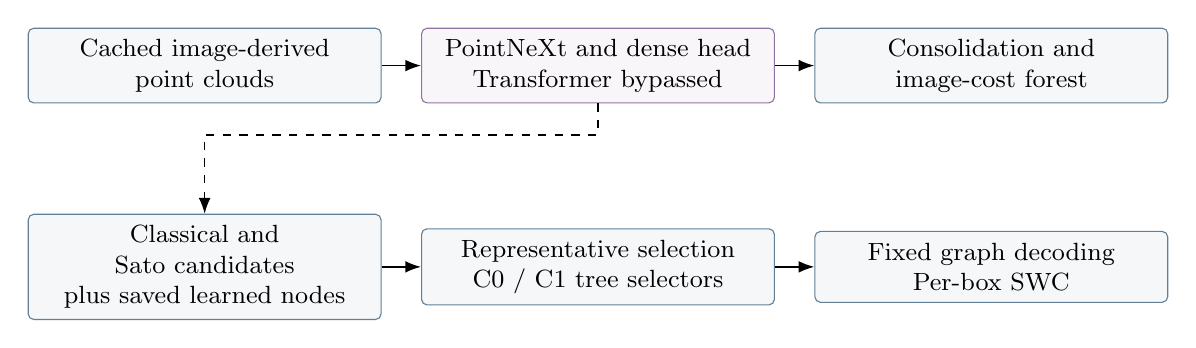
\begin{tikzpicture}[node distance=9mm and 5mm]
\node[stage,text width=42mm] (points) {Cached image-derived\\point clouds};
\node[learning,right=of points,text width=42mm] (dense) {PointNeXt and dense head\\Transformer bypassed};
\node[stage,right=of dense,text width=42mm] (forest) {Consolidation and\\image-cost forest};
\node[stage,below=14mm of points,text width=42mm] (pool) {Classical and Sato candidates\\plus saved learned nodes};
\node[stage,right=of pool,text width=42mm] (trees) {Representative selection\\C0 / C1 tree selectors};
\node[stage,right=of trees,text width=42mm] (decode) {Fixed graph decoding\\Per-box SWC};
\draw[arr] (points)--(dense);\draw[arr] (dense)--(forest);
\draw[arr] (pool)--(trees);\draw[arr] (trees)--(decode);
\draw[arr,dashed] (dense.south) -- ++(0,-4mm) -| (pool.north);
\end{tikzpicture}
\caption{The two experimental paths actually tested. The later selectors reused saved learned positions together with classical and Sato candidates; they did not train a new proposal model. Both paths were evaluated per box. GATv2 and whole-image assembly were not reached.}
\label{fig:actual}
\end{figure}

The four-box model fitted its training examples well by the segment metric, but transferred poorly. That result motivated the broader training run: the head had initially seen only two neurons, which was not enough to judge its behavior across the cohort. The broad run used all 460 training boxes from 33 neurons for 20 epochs, ending at 9,200 updates. It retained the frozen 2,048-point inputs; the higher-count input audit was not itself a successful reconstruction experiment.\evidence{transfer,broad}

\begin{table}[htbp]
\centering
\caption{What broader training changed for the dense head. Values are segment F1 at two voxels, in percent. The rows describe different training cohorts, not repeated runs of the same experiment.}
\begin{tabular}{lrr}
\toprule
Dense-head experiment & Training & Development\\
\midrule
Four-box fit & 81.49 & 23.20\\
Broad 33-neuron run & 37.84 & 36.04\\
\bottomrule
\end{tabular}
\label{tab:training}
\end{table}

The broader run recovered a substantial amount of candidate geometry. At two voxels, candidate-edge coverage increased from 38.07\% for the four-box model to 81.69\%. Development recall reached 74.40\%, but precision was only 24.80\%. The model had become better at reaching the reference while still producing too much other geometry.\evidence{transfer,broad}

The training and development F1 values in Table~\ref{tab:training} are both low for the broad run. This is important: the broad result cannot be explained simply by repeating the earlier small-fit transfer gap. Under the fixed recipe, useful localization and selection remained inadequate even across the training cohort. The experiment does not isolate whether the limiting factor was supervision, features, optimization or reference completeness.

I stopped that recipe after it failed the predeclared comparison. The required development segment F1 was 59.33\% at two voxels and 74.14\% at six, with wins over the matched classical control on at least five of seven neurons at each tolerance. The broad head reached 36.04\% and 67.54\%, with two and three neuron wins.\evidence{broad}

This was a 20-epoch \emph{dense-head} run. It was not a 20-epoch Transformer experiment, and it cannot establish that Transformer set prediction is either undertrained or incapable of working.

\section{Moving from node agreement to reconstruction quality}
\subsection{Why the scorer had to follow the graph}
The diagram places connectivity after proposal generation, so isolated-node agreement could not be the only measure. A segment between two nodes can represent a branch even when there is no node at every location. At the same time, a dense collection of paths can remain close to the reference while containing many redundant samples.

I therefore retained two complementary measurements. Segment F1 measures arclength agreement with continuous curves, at two and six native voxels. Resampled F1 first samples the skeletons uniformly at two-voxel arclength spacing, then uses maximum-cardinality one-to-one matching within the chosen tolerance. The length ratio records predicted arclength divided by reference arclength. Together they make excess structure and missing coverage more visible. Neither geometric F1 certifies the correctness of every branch connection.\evidence{formulation,compact}

The original scores were preserved when the additional metrics were added. This was an extension of the measurement, not a retrospective conversion of failed gates into passes.

\subsection{The controls and the stronger archive comparison}
The main controls were an image-only classical graph and a Sato-ranked point forest. The classical graph used the preserved automatic thresholding, skeletonization and pruning recipe. The Sato arm selected strongly ranked image points and used a fixed consolidation/forest procedure. These controls helped establish whether learning added value beyond the structure already encoded by preparation.

Later, I recovered the BigNeuron archive outputs for the same seven development neurons. The strongest fixed archive variant across these neurons was labelled \texttt{neutube\_updated}. This is a descriptive leader selected from the inspected development comparison, not a comparator chosen on training data before our experiments. The archive is parameter-optimized and its seed provenance is unresolved. It is useful context, but I would not present it as a reproduced, independently configured deployment baseline.\evidence{benchmark}

\begin{table}[htbp]
\centering
\caption{Matched development comparison on seven neurons and 151 reference-present boxes. F1 values are percentages; length is pooled predicted/reference arclength. ``Broad dense'' is our terminal 33-neuron head, not the Transformer.}
\label{tab:main}
\small
\setlength{\tabcolsep}{5pt}
\begin{tabular}{lrrrrr}
\toprule
& \multicolumn{2}{c}{Segment F1} & \multicolumn{2}{c}{Resampled F1} & Length\\
\cmidrule(lr){2-3}\cmidrule(lr){4-5}
System & 2 vox & 6 vox & 2 vox & 6 vox & ratio\\
\midrule
\DevelopmentMacroRows
\bottomrule
\end{tabular}
\par\smallskip
\begin{minipage}{\linewidth}\footnotesize
\textsuperscript{*}The archive leader's Series017 case is a whole-case protocol zero under the frozen bounds check. Its actual supplied trace has not been shown to have zero overlap. The exact pooled ratio is 1.25017, slightly above 1.25; rounding is not a pass. Per-neuron values are in Appendix~\ref{app:neurons}.
\end{minipage}
\end{table}

\begin{figure}[htbp]
\centering
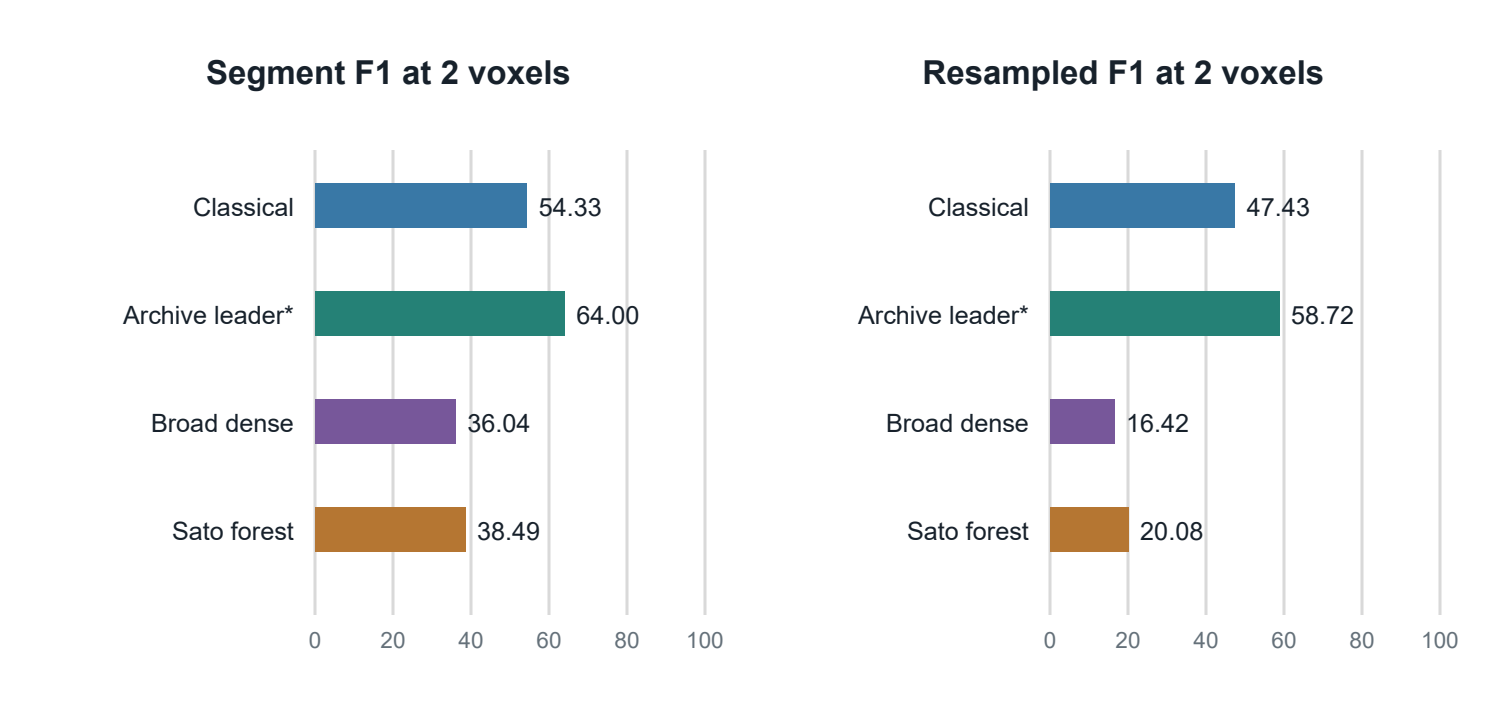
\includegraphics[width=\linewidth]{development_comparison.png}
\caption{The same saved development reconstructions evaluated at two voxels. The resampled metric exposes excess geometry in both the broad dense head and the Sato forest. These are the numerical rows in Table~\ref{tab:main}, not additional experiments.}
\label{fig:main}
\end{figure}

The broad head's 6.24-fold length is especially informative. Its segment score gives some credit for reaching much of the reference, but its one-to-one resampled score is only 16.42\% at two voxels. The Sato forest has a similar length problem. The classical graph is incomplete on several neurons, yet provides a more compact reconstruction under the same measurement.\evidence{compact}

For me, this changed the immediate question. We needed to understand which candidate structure should survive, and whether the graph stage could preserve weak branches without retaining a large amount of unrelated or duplicate geometry.

\subsection{The coordinate limitation in the archive result}
The recovered archive contains 237 outputs across 44 implementation/mode variants. Across the seven-neuron grid, 208 method/case slots passed the structural and bounds checks, 71 were missing, and 29 supplied files were rejected. Missing or rejected entries remained zeros rather than being removed from the comparison.\evidence{benchmark}

One of those zeros particularly affects the interpretation of the best archive variant. Its Series017 file contains 16 nodes; one lies just 0.2044 voxel beyond the native voxel-cell boundary. That fails the frozen requirement that at least 99\% of vertices lie inside the bounds, so the whole case scores zero. This is an overly coarse screen for distinguishing a small endpoint overshoot from a coordinate-frame mismatch. Passing it also does not establish the subvoxel origin.

I have kept the frozen result visible rather than silently relaxing the rule after seeing which method it affected. A boundary-sensitivity analysis or a reference-offset correction would need a separately defined protocol. The current comparison remains provisional, and no neuron has been excluded because of this issue.\evidence{benchmark}

\section{What the candidate and graph experiments revealed}
\subsection{The early oracle looked stronger than the compact reconstruction}
Before training a graph selector, I asked whether the candidate pool contained enough useful structure at all. The pool combined classical vertices and edges, Sato candidates and saved broad-head nodes. An oracle used the reference to score candidate choices before decoding. Its purpose was to measure geometric opportunity, not ordinary inference performance.

The first union-oracle score was 90.42\% segment F1 at two voxels. That passed the original headroom criterion, but it did so at approximately 2.40 times the reference length. Once the resampled scorer was added, its two-voxel F1 was only 41.49\%. The interpretation of that early pass therefore needed correcting.\evidence{compact}

With a fixed duplicate-handling step before spanning, the compact union oracle reached 88.52\% segment F1, 64.80\% resampled F1 and 1.185 times the reference length. It gave up a small amount of segment overlap while becoming much less redundant. The remaining gap between the two scores is one reason I do not treat high segment overlap as a complete reconstruction result.

\begin{table}[htbp]
\centering
\caption{Reference-assisted development diagnostics. These use reference information unavailable to a real inference system. The first two rows test candidate selection and compaction; the last two start from the preserved classical graph and test editing opportunity.}
\label{tab:oracle}
\small\setlength{\tabcolsep}{5pt}
\begin{tabular}{lrrrrr}
\toprule
& \multicolumn{2}{c}{Segment F1} & \multicolumn{2}{c}{Resampled F1} & Length\\
\cmidrule(lr){2-3}\cmidrule(lr){4-5}
Reference-assisted method & 2 vox & 6 vox & 2 vox & 6 vox & ratio\\
\midrule
\OracleRows
\bottomrule
\end{tabular}
\end{table}

\subsection{Why simpler selectors came before GATv2}
The next test used gradient-boosted trees before GATv2, so that a failure in candidate representation or labels would not immediately be attributed to a more complex graph network. I compared two contracts on the same image-only representative graph. C0 retained the original dense-pool adjacency labels. C1 recomputed the adjacency target after representative selection.\evidence{trees}

\begin{table}[htbp]
\centering
\caption{CPU selector results from conditional leave-neuron-out CV across the 33 training neurons. F1 values are percentages. These are not seven-neuron development scores.}
\small\setlength{\tabcolsep}{7pt}
\begin{tabular}{lrrrrr}
\toprule
& \multicolumn{2}{c}{Segment F1} & \multicolumn{2}{c}{Resampled F1} & Length\\
\cmidrule(lr){2-3}\cmidrule(lr){4-5}
Contract & 2 vox & 6 vox & 2 vox & 6 vox & ratio\\
\midrule
C0 & 51.32 & 82.47 & 39.41 & 55.88 & 1.255\\
C1 & 58.49 & 83.72 & 40.85 & 55.06 & 1.740\\
\bottomrule
\end{tabular}
\end{table}

C1 improved segment overlap, which supports the importance of matching labels to the actual representative graph. However, resampled agreement remained weak and the length increased. Both contracts exceeded the fixed 1.25-fold pooled length limit; C0's unrounded value was 1.254998. I stopped at that point. The final selector development comparison, PointNeXt edge-feature comparison and GATv2 training were not reached.\evidence{trees}

The CV was conditional on the frozen upstream system: candidate positions and encoder features had already been trained using all 33 training neurons. The selectors left out each neuron in turn, but this was not a strict cross-fitted evaluation of the entire pipeline. It cannot establish complete-pipeline generalization.

\subsection{The image review made the failures easier to interpret}
The saved review sheets showed that the same aggregate problem could arise in different ways. On WED\_SLP, diffuse image structure attracted many retained candidates and decoded paths beyond the supplied trace. On an adult zebrafish example, the reference followed dim branches that were poorly represented in the retained output. Figure~\ref{fig:review} places those cases next to the image evidence.\evidence{post}

This is why I would not explain the current results with one global statement about an inadequate encoder, missing input points or bad annotations. In some cases the system retains too much; in others it loses weak structure. The review does not isolate the causal stage, but it gives us concrete problems to test. It also gives the proposed include/exclude interaction a clearer purpose.

\begin{figure}[p]
\centering
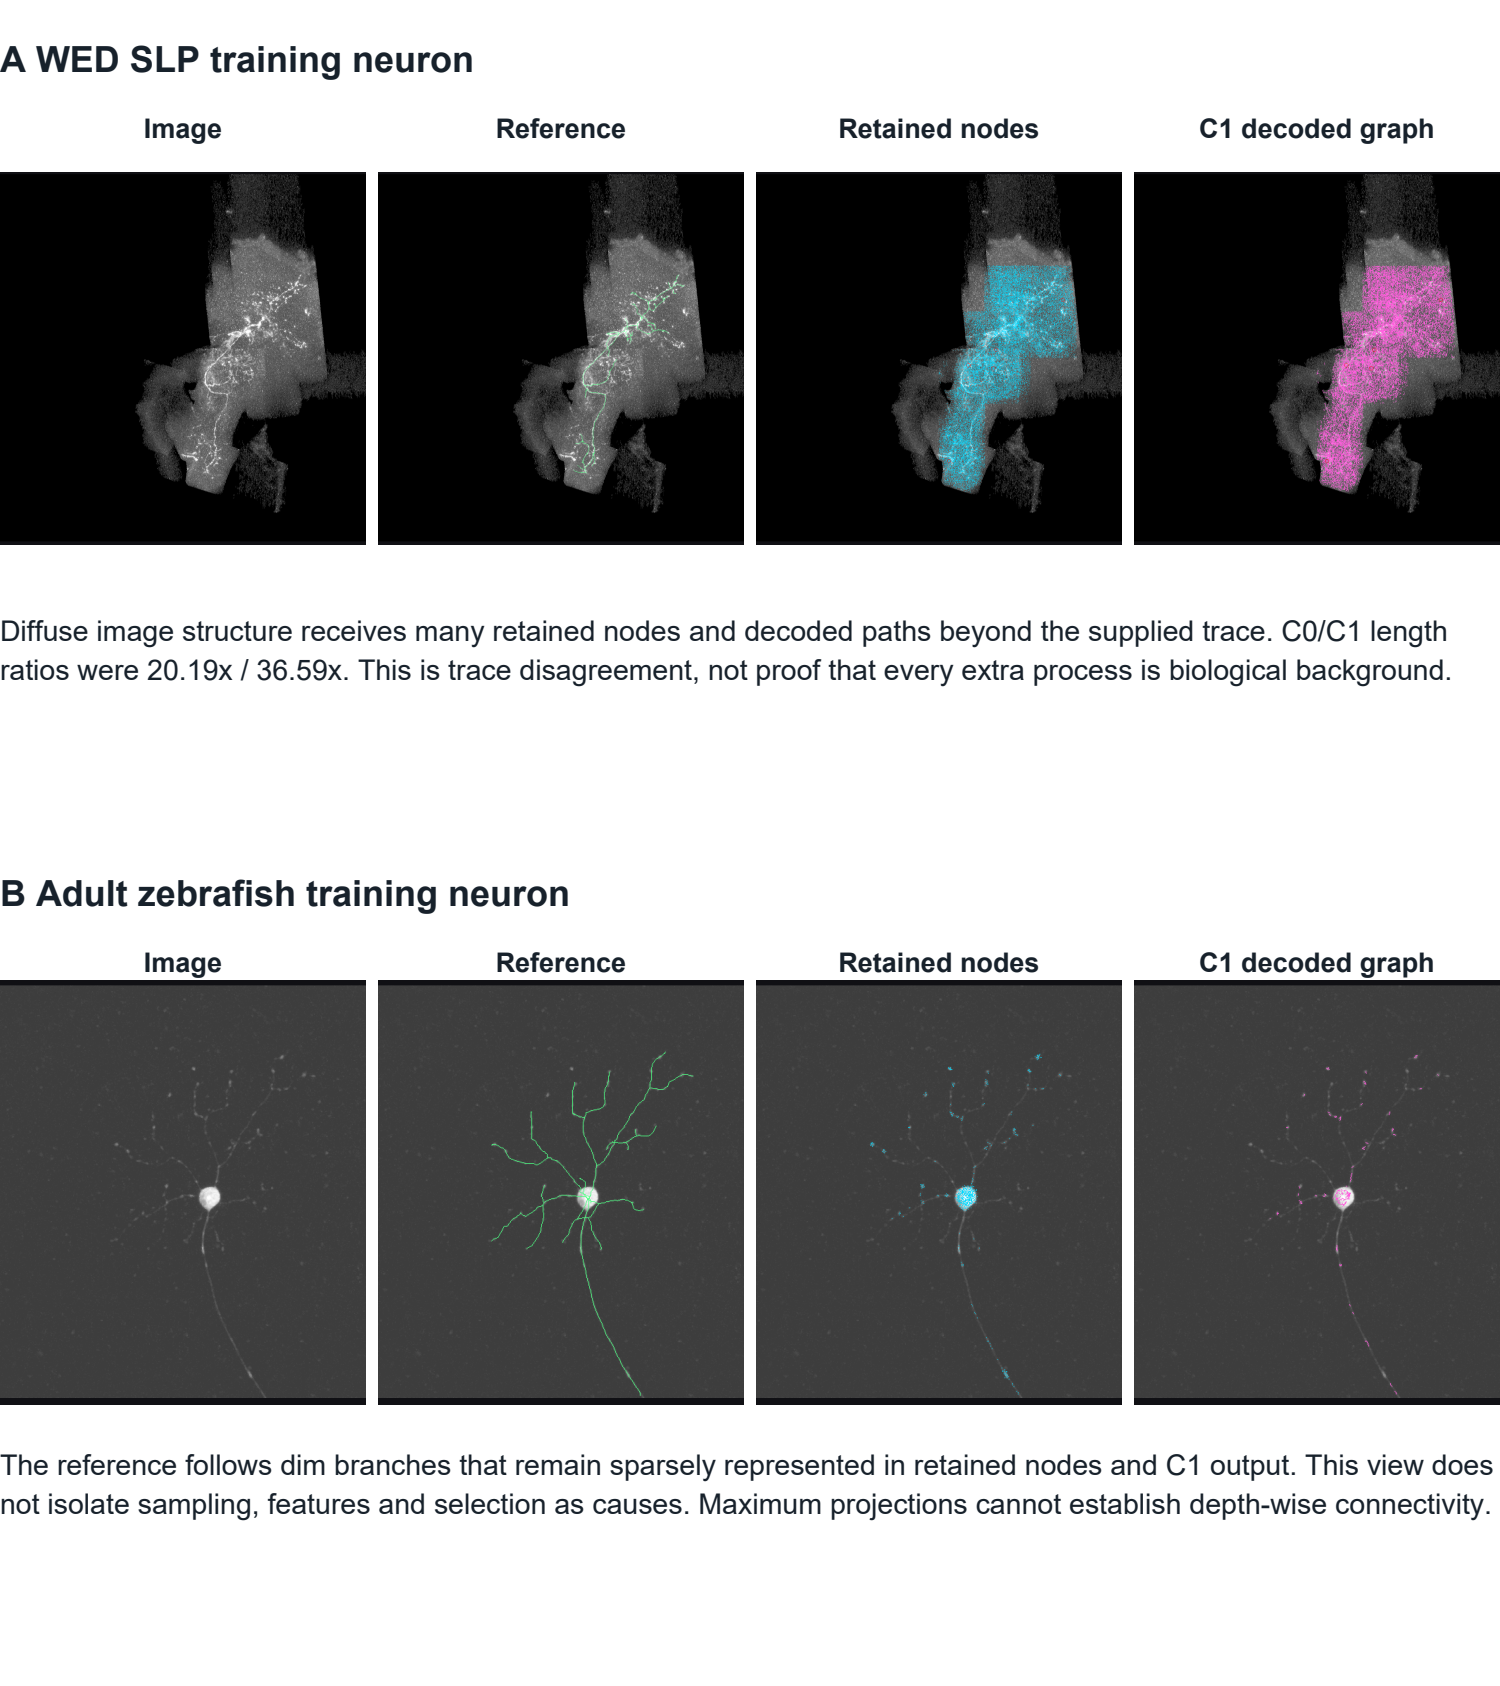
\includegraphics[width=\linewidth]{saved_review_examples.png}
\caption{Two illustrative training neurons from the saved review. Green is the supplied reference, cyan the retained nodes and magenta the C1 decoded graph. WED\_SLP illustrates excess retained structure; the adult zebrafish example illustrates loss of dim branches. These are selected diagnostic examples, not a random sample. The full-resolution original sheets are included in the report folder. Maximum projections do not establish depth-wise connectivity or prove that every untraced process is biological background.}
\label{fig:review}
\end{figure}

The broader gold-to-ridge diagnostic also needs this care. Across the 40 measured neurons, 16.60\% of pooled training reference length and 15.06\% of development reference length lay more than two voxels from the fixed intensity-ridge proxy. Weak or discontinuous image signal can cause that proxy to miss a branch. These offsets are therefore evidence to inspect, not grounds for declaring the gold wrong or relabeling the data.\evidence{post}

\subsection{Classical editing remains an opportunity rather than a result of learning}
The final headroom test began with the classical graph itself. A reference-assisted prune-only procedure reached 58.58\% resampled F1 at two voxels. Allowing connected additions from the other candidates raised that to 61.74\%. This cleared the agreed 60\% threshold for drafting an editing formulation. It did not qualify a learned model.\evidence{post}

The achieved score also needs to be read alongside the search limit. The prune-plus-add search reached its 128-edit cap in 106 of 151 boxes; 97 boxes then used component drops to meet the length budget. It is a feasible result of that bounded search, not the maximum quality available from the candidate pool.

Against the archive leader, the apparent resampled margin is only 3.02 percentage points at two voxels and 0.40 at six, and it depends on the Series017 protocol zero. I would therefore keep classical-anchored editing as a discussion draft. The evidence supports examining a better-defined task, but not claiming that this particular editing recipe has already secured a large advantage.\evidence{benchmark}

\section{Returning to the semi-automatic part of the idea}
The original interaction idea now has a more specific question behind it. If a user can mark a dim region that preparation missed, or a distracting area that receives too many points, can that small intervention improve the reconstruction? More importantly, can the accumulated corrections improve preparation on later neurons from the same acquisition conditions?

Those are two separate capabilities. Recomputing the current image after a stroke can be useful even without learning. A laboratory-specific model would need to learn from earlier corrections and improve a different neuron that has not been corrected. Saving the strokes alone would not make the current fixed Sato guide adaptive.

I would want the interaction to remain coarse. The user should see the raw image with evidence overlays and linked views, rather than being asked to draw the final skeleton. An include stroke could increase sampling or supply image-derived candidates around a missed process. An exclude stroke could reduce attention to distracting structure. The model would still have to use the image to determine the actual geometry and connections.

This also means the front end cannot be evaluated in isolation. If a later selector discards the extra evidence, an improved preparation does not produce a better neuron. The fixed downstream control in the proposed study is intended to make that visible before we introduce another learned head.

\begin{figure}[htbp]
\centering
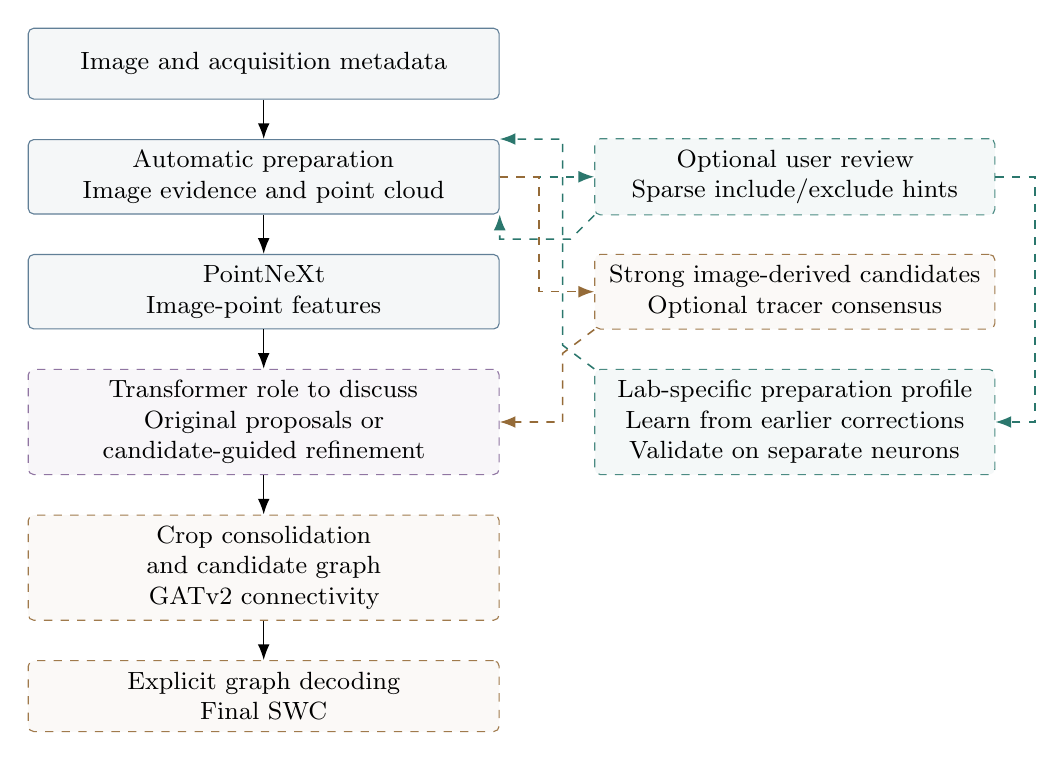
\begin{tikzpicture}[node distance=5mm and 12mm]
\node[stage] (im) {Image and acquisition metadata};
\node[stage,below=of im] (prep) {Automatic preparation\\Image evidence and point cloud};
\node[feedback,right=12mm of prep,text width=48mm] (review) {Optional user review\\Sparse include/exclude hints};
\node[stage,below=of prep] (enc) {PointNeXt\\Image-point features};
\node[planned,right=12mm of enc,text width=48mm] (cand) {Strong image-derived candidates\\Optional tracer consensus};
\node[learning,below=of enc,dashed] (trans) {Transformer role to discuss\\Original proposals or\\candidate-guided refinement};
\node[feedback,right=12mm of trans,text width=48mm] (profile) {Lab-specific preparation profile\\Learn from earlier corrections\\Validate on separate neurons};
\node[planned,below=of trans] (graph) {Crop consolidation and candidate graph\\GATv2 connectivity};
\node[planned,below=of graph] (swc) {Explicit graph decoding\\Final SWC};
\draw[arr] (im)--(prep);\draw[arr] (prep)--(enc);\draw[arr] (enc)--(trans);
\draw[arr] (trans)--(graph);\draw[arr] (graph)--(swc);
\draw[arr,dashed,pnteal] (prep)--(review);
\draw[arr,dashed,pnteal] (review.south west) -- ++(-3mm,-3mm) -| (prep.south east);
\draw[arr,dashed,pnteal] (review.east) -- ++(5mm,0) |- (profile.east);
\draw[arr,dashed,pnteal] (profile.north west) -- ++(-4mm,3mm) |- (prep.north east);
\draw[arr,dashed,pnorange] (prep.east) -- ++(5mm,0) |- (cand.west);
\draw[arr,dashed,pnorange] (cand.south west) -- ++(-4mm,-3mm) |- (trans.east);
\end{tikzpicture}
\caption{A possible direction for discussion. Dashed paths and boxes show proposed or unbuilt work. Corrections can help the current image, while a validated lab profile would guide preparation on later images. PointNeXt, the Transformer and GATv2 remain visible research roles; the Transformer choice is unresolved. Reference SWCs would supervise training and score outputs, not generate inference candidates or roots.}
\label{fig:proposed}
\end{figure}

My inclination is to begin with a simulated-user experiment on training neurons, before asking anyone to mark the cohort. The same bounded include/exclude actions would be compared with output proofreading under a fixed downstream method. A zero-correction arm would show the automatic starting point. Adaptation would be assessed on other neurons within an acquisition group, with unmarked regions kept unknown.

That simulation would establish whether sparse guidance has enough potential to justify building the interaction system. Gold-directed placement is privileged: it avoids the real user's problem of finding the error. Jittering a hint does not reproduce that search effort. Stroke length and width would also need limits, so one ``correction'' could not quietly reveal an entire branch. Real user time and usability would remain a later question.

Consensus over strong tracers is another candidate source to examine, especially now that the archive is available. However, consensus, a contextual Transformer and GATv2 should each be compared against a simpler alternative. I would not add them all at once and then attribute a combined improvement to the point-based model.

\clearpage
\section{The decisions I would like to discuss with you}
The work has brought me back to the original aim with a clearer account of what is missing. We have a working way to prepare, train and measure the components, and some encouraging evidence that the small geometric task is learnable. We do not yet have a learned reconstruction that outperforms the strongest available automatic reference on the inspected development cohort. I would like the next experiment to answer a focused research question rather than simply extend a recipe that has already failed its comparison.

There are five points on which your guidance would be especially useful:
\begin{enumerate}
\item \textbf{The role of interaction.} Would you be comfortable making the lab-adaptive, semi-automatic front end part of the central PN2 question? I would keep automatic performance, benefit on a corrected image, and transfer to later uncorrected images as separate results.
\item \textbf{The candidate-based framing.} Is learning to refine strong image-derived candidates an acceptable development of the original idea? The experimental dense-head arm already bypassed Transformer proposals, but I have not adopted that departure as the project architecture. I would like your agreement before taking it further.
\item \textbf{A useful role for the Transformer and GATv2.} Would you prefer to retain independent Transformer node proposals, investigate candidate-guided refinement, or compare those two roles? GATv2 remains the intended connectivity model; it has not yet been trained. We should decide what improvement over simpler selection and decoding would justify each model.
\item \textbf{The evaluation we should trust.} Can we agree on a coordinate/QC protocol and a prospective combination of segment agreement, one-to-one resampled agreement, length and topology checks? The current bounds-screen issue should be resolved transparently, with full-cohort results retained rather than selecting favorable neurons.
\item \textbf{The next bounded experiment.} My preference would be to test sparse guidance and within-group transfer first, while keeping stronger tracer-consensus headroom as a separate comparison. Does that match your priorities, and what should be frozen before we eventually use the untouched reserved cohort?
\end{enumerate}

\clearpage
\appendix
\section{How the measurements should be read}
\label{app:metrics}
The development results score the same 151 reference-present boxes from the seven named neurons. Whole-image assembly has not been completed. A good per-box result therefore does not establish correct merging across crop boundaries, biological roots or anatomical radii.

Segment scoring uses directed arclength precision and recall against continuous polylines, with a maximum quadrature step of 0.5 native voxel. Resampled scoring uses skeleton samples at two-voxel arclength spacing and maximum-cardinality bipartite matching at the reported two- or six-voxel tolerance. Both are measures of agreement with the supplied traces, not exhaustive biological foreground or complete topology scores.

Box statistics are pooled within each neuron before its precision, recall and F1 are computed. The development headline F1 is the mean of the seven neuron F1 values. It is not recomputed from macro precision and recall. The headline length ratio pools predicted and reference lengths over the cohort; Appendix~\ref{app:neurons} instead gives each neuron's ratio.

Micron-scale diagnostic views are available in the saved ridge results where reported spacing exists. They remain conditional on that calibration. The tables in this report use native voxel tolerances throughout, without implying a uniform physical accuracy across acquisitions.

Reference-empty boxes were treated as annotation-unknown, not background. The 1,504 training and 264 development boxes outside the reference-present scoring set remain part of the image domain, but are not included in the comparison tables. Their exclusion from these diagnostic tables is a scoring scope, not an inference policy that can consult the gold.

Execution checks included source/packet hashes, point coordinate and intensity provenance, scorer fixtures, train/evaluation consistency, exposure counts and checkpoint/optimizer verification. The complete saved record remains available. These checks support reproducibility; they do not convert a fit or an oracle into a learned reconstruction improvement.\evidence{cohort,formulation,broad,compact}

\clearpage
\section{All seven development neurons}
\label{app:neurons}
The following table contains all 28 method/neuron rows. F1 values are percentages, and the length ratio is predicted/reference arclength within that neuron's scored boxes. Full case identities and unrounded values are provided in \texttt{development\_results.csv}.\evidence{compact,benchmarkdata}

\begingroup\fontsize{9.5}{11.5}\selectfont
\renewcommand{\arraystretch}{1.0}
\setlength{\tabcolsep}{6pt}
\begin{longtable}{lrrrrr}
\caption{Per-neuron development results for the four comparison systems.}\label{tab:neurons}\\
\toprule
& \multicolumn{2}{c}{Segment F1} & \multicolumn{2}{c}{Resampled F1} & Length\\
\cmidrule(lr){2-3}\cmidrule(lr){4-5}
System & 2 vox & 6 vox & 2 vox & 6 vox & ratio\\
\midrule\endfirsthead
\multicolumn{6}{l}{\small Table~\thetable\ continued}\\
\toprule
System & Seg 2 & Seg 6 & Res 2 & Res 6 & Length ratio\\
\midrule\endhead
\midrule\multicolumn{6}{r}{\footnotesize Continued on the next page}\\\endfoot
\bottomrule\endlastfoot
\DevelopmentNeuronRows
\end{longtable}
{\footnotesize\textsuperscript{*}Series017 is a protocol zero for the archive leader because of the native-bounds screen, including its length contribution. This does not describe the supplied SWC's actual overlap or length. No development neuron was removed from any reported aggregate.}
\endgroup

\clearpage
\section{Saved source records and access}
The public repository is \url{https://github.com/GraphiCortex/PointNeuron_Rec}. The report package is on branch \texttt{pointneuron2}, under \texttt{docs/reports/progress\_20261107/}. Evidence links below are pinned to commit \texttt{8c363d3}.

Local paths are relative to {\small\nolinkurl{C:/Users/Seywe/Documents/GitHub/PointNeuron/PN2/}}. This is the branch's Git root: GitHub paths begin with \texttt{docs/}, not \texttt{PN2/docs/}. The figures and portable evidence are tracked; full caches and checkpoints under \texttt{tmp/} remain local.

\begingroup\footnotesize
\begin{thebibliography}{99}
\setlength{\itemsep}{2pt}
\setlength{\parskip}{0pt}
\bibitem{pointneuron} R. Zhao, H. Wang, C. Zhang and W. Cai. \emph{PointNeuron: 3D Neuron Reconstruction via Geometry and Topology Learning of Point Clouds}. WACV 2023. \url{https://arxiv.org/abs/2210.08305}. Conceptual starting point; no PN1 result is used as a fresh PN2 measurement here.
\bibitem{design} Proposal-to-implementation audit, including the original architecture and its experimental departures.\par\sourcepath{docs/proposal_implementation_audit_20261104.md}
\bibitem{cohort} Cohort capacity and supervision preflight.\par\sourcepath{docs/node_cohort_preflight_results.md}
\bibitem{support} Saved two-voxel input-support measurements.\par\sourcepath{docs/evidence/curve_transfer_input_support_20261104.json}
\bibitem{transformer} Geometric-query Transformer four-box fit.\par\sourcepath{docs/geometric_query_fit_results.md}
\bibitem{formulation} Curve formulation audit and scorer controls.\par\sourcepath{docs/curve_formulation_audit_results.md}
\bibitem{transfer} Four-box dense-head development transfer.\par\sourcepath{docs/curve_transfer_development_results_20261104.md}
\bibitem{broad} Broad dense-head terminal results and fixed comparison.\par\sourcepath{docs/broad_curve_head_results_20261105.md}
\bibitem{compact} Saved segment/resampled metrics and compact-oracle measurements.\par\sourcepath{docs/evidence/resampled_compact_completed_20261105.json}\par\sourcepath{docs/resampled_compact_results_20261105.md}
\bibitem{trees} Stopped CPU selector comparison and conditional-CV limitations.\par\sourcepath{docs/stage2_trees_results_20261106.md}\par\sourcepath{docs/evidence/stage2_trees_stopped_20261106.json}
\bibitem{post} Image review, ridge diagnostics and classical-anchored editing.\par\sourcepath{docs/post_stage2_diagnostics_results_20261106.md}\par\sourcepath{docs/evidence/post_stage2_diagnostics_completed_20261106.json}
\bibitem{benchmark} Recovered BigNeuron archive comparison and coordinate limitation.\par\sourcepath{docs/bigneuron_benchmark_results_20261106.md}\par\sourcepath{docs/evidence/bigneuron_benchmark_completed_20261106.json}
\bibitem{benchmarkdata} Archive per-neuron measurements.\par\sourcepath{docs/evidence/bigneuron_per_neuron_20261106.csv}
\bibitem{editing} Classical-anchored editing contract, discussion draft only.\par\sourcepath{docs/classical_anchored_editing_contract_DRAFT_20261106.md}
\end{thebibliography}
\endgroup
\end{document}
